\documentclass[11pt]{article}
\usepackage{lingmacros}
\usepackage{tree-dvips}
\usepackage{titlesec}

\usepackage[utf8]{inputenc}
\usepackage[nottoc,numbib]{tocbibind}
\usepackage[T1]{fontenc}
\usepackage{lmodern}
\usepackage[ngerman]{babel}
\usepackage{amsmath, amssymb, amscd, amsthm, amsfonts}
\usepackage{sectsty}
\usepackage{titling}
\usepackage{glossaries}
\usepackage{listings}
\usepackage{xcolor}
\usepackage{graphicx}
\usepackage{tikz}
\usepackage{tikz-qtree}
\usepackage[ngerman]{babel}
\usepackage{verbatim}
\usepackage[bottom]{footmisc}
\usepackage[export]{adjustbox}
%graphics


%definition the colors 
\definecolor{olive}{RGB}{128,128,0}
\definecolor{gray}{rgb}{0.5,0.5,0.5}
\definecolor{lightSteelBlue}{RGB}{240,240,240}
\definecolor{crimson}{RGB}{220,20,60}
\definecolor{niceBlue}{RGB}{0,210,210}


%listdefinition for C code
\lstdefinestyle{ColorStyle}{
    backgroundcolor=\color{lightSteelBlue},   
    commentstyle=\color{olive},
    keywordstyle=\color{crimson},
    numberstyle=\tiny\color{gray},
    stringstyle=\color{niceBlue},
    basicstyle=\ttfamily\footnotesize,
    breakatwhitespace=false,         
    breaklines=true,                 
    captionpos=b,                    
    keepspaces=true,                 
    numbers=left,                    
    numbersep=5pt,                  
    showspaces=false,                
    showstringspaces=false,
    showtabs=false, 
    language=C,  
    tabsize=2
}

%command list
\renewcommand{\abstractname}{Summary}
\newcommand{\qt}{Quadtree }
\newcommand{\oc}{Octree }
\newcommand{\kd}{KD-Tree }
\newcommand{\qts}{Quadtrees }
\newcommand{\ocs}{Octrees }
\newcommand{\kds}{KD-Trees } 
\newcommand{\nw}{northWest}
\newcommand{\noea}{northEast}
\newcommand{\sw}{southWest}
\newcommand{\se}{southEast}
\newcommand{\fett}[1]{{\bf #1}}
\newcommand\blueColor[1]{\color{niceBlue}#1}
\newcommand{\lstin}[1]{\lstinline[language=C]{#1}}

%title settings
\renewcommand\maketitlehooka{\null\mbox{}\vfill}
\renewcommand\maketitlehookd{\vfill\null}

\oddsidemargin 0pt
\evensidemargin 0pt
\marginparwidth 40pt
\marginparsep 10pt
\topmargin -20pt
\headsep 10pt
\textheight 8.7in
\textwidth 6.65in
\linespread{1.2}

%deckblatt 
\title{\textbf{Tree Data Structures: Quad-/Oc-/KD-Trees}}
\author{Siobhan-Lillian Hönig}
\date{\today}

%glossary einträge
\makeglossaries
\newglossaryentry{B}{
    name={Baumstruktur},
    description={Baumstrukturen sind Strukturen, die sowohl aus sogenannten Knoten und Kanten bestehen, als auch aus inneren Knoten und Blättern. Graphisch betrachtet, ähneln sie einem Baum, deshalb auch die Namensgebung. Baumstrukturen werden oftmals verwendet, sobald in einer großen Datenmenge ein bestimmtes Element gesucht wird}}

\newglossaryentry{R}{
    name={Root},
    description={Root: aus dem Englischen übersetzt = wurzel. Im programmieren wird dieser Begriff im Hinblick auf Baumstrukturen als Ursprungsknoten bezeichnet. Alle nachfolgenden Knoten erben von diesem}}

\newglossaryentry{N}{
    name={Node},
    description={Node ist die englische Bezeichung für Knoten. Baumstrukturen bestehen aus einem Aufbau von Knoten, wobei der Ursprungsknoten die Wurzel ist. Folgt nach den Knoten ein weiterer, handelt es sich um einen inneren Knoten.}}

\newglossaryentry{L}{
    name={Leaf oder auch Blatt},
    description={Leaf oder auch Blatt: Äußere Knoten sind Knoten, welche keine Kinderknoten besitzen und somit das "Ende" des Baumes angeben.}}

\newglossaryentry{CN}{
    name={ChildrenNode},
    description={Children Nodes sind Knoten, welche von ihren parent nodes Daten erben. Alle nodes, welche Daten der root erben, sind die children nodes des Baumes}}

\newglossaryentry{BinBa}{
    name={Binärer Baum},
    description={ diese Baumstruktur von anderen Strukturen unterscheidet ist die Anzahl der Nachkommen. Hier ist die Anzahl auf zwei Knoten begrenzt. }}

\newglossaryentry{Malloc}{
    name={Malloc},
    description={Ist eine Speicherallokierung genutzt um während der Programlaufzeit (dynamisch) Speicherplatz zur Verfügung zu stellen. Dies ist vor allem nützlich, wenn unbekannt ist, wieviel Speicher benötigt wird. Wenn der Speicher nicht mehr genutzt wird, kann mit dem free() Operator der Speicher wieder freigegeben werden.}}

\newglossaryentry{rekursiv}{
    name={rekursiv},
    description={Rekursive Strukturen sind Strukturen in denen die Datenmengen gleich groß sind und durch Referencen verknüpft sind, z.b. Baumstrukturen}}

\newglossaryentry{balanciert}{
    name={Ausbalancierter Baum},
    description={Bei Baumstrukturen kann es vorkommen,dass sich einer der Unterbäume sehr in die Baumtiefe ausbreitet und bei Suchanfragen es zu langen Warteschlangen kommt. Um dies vorzubeugen werden ausbalancierte Strukturen generiert. Diese beugen solche Probleme vor}}

\newglossaryentry{GIS}{
    name={GIS},
    description={Das Geografische Informationssystem wird genutzt um Daten mit einer Karte zu verbinden und diese Positionsdaten mit beschreibenden Informationen zu versehen. }}

    \newglossaryentry{ConquerandDivide}{
        name={Conquer and Divide},
        description={Teile und Herrsche ist ein Verfahren, das oftmals für Such- und Sortierverfahren genutzt wird. Kurz gesagt, wird ein größeres Problem in kleinere zerlegt und diese einzeln bearbeitet. Die Unterteilung erfolgt hier rekursiv. Aus den Teilegebnissen wird  anschließend ein Ergebnis konstruiert.}}

%sets the style used for the listings 
\lstset{style=ColorStyle}

%start of document
\begin{document}

\begin{titlepage}
    \maketitle
\end{titlepage}

\pagebreak

\pagebreak
\tableofcontents
\pagebreak



%glossary
\glsaddall
\printglossary[title=Special terms, toctitle=List of terms]
\pagebreak

\section{Einführung} \label{Einführung}

Mit der Weiterentwicklung von rechenfähigen Computern wurde zum einen der mögliche Speicherplatz für Daten immer größer, zum andern die Datenmengen umfangreicher. Um diese Daten besser zu sortieren und um schneller darauf zugreifen zu können, wurden und werden sogenannte Datenstrukturen genutzt. Die Daten werden in bestimmten Formen gespeichert, der Aufbau dieser Strukturen kann so z.B.einem Graph aber auch einem Baum ähneln. 
In dieser Seminarabeit werden Baumstrukturen erklärt. Aufgrund dessen, dass die Informatik sehr aufgefächert ist, sind sehr viele Spezifikationen der Bäume für bestimmte Datenmengen entstanden.  
Wie bereits erwähnt ermöglichen Datenstrukturen eine effiziente Suche der Daten, ich werde drei dieser Baumstrukturen vorstellen, erklären, sowie betrachten, wie effizient sie in bestimmten Situationen sind. 
\newline
Allgemein sind Baumstrukturen wie der Name schon besagt, hierarchische Datenstrukturen deren Aufbau dem eines Baumes ähnelt. Sie besitzen eine Wurzel, auch root genannt und jeweils nodes (Knoten) welche die children/ Kinder von der root oder der jeweiligen parent node sind.  In diesen nodes können Daten gespeichert werden, dies ist aber nicht zwingend. In manchen Fällen ist es auch gewünscht, nichts zu speichern.  
In dieser Arbeit wird es um diese drei Baumstrukturen gehen: \fett \qt ,\fett \oc und \fett \kd. Diese werden für unterschiedliche Zwecke und Situationen verwendet. Zum einen um Punkte in einem 2-D Raum, 3.D Raum oder sogar in mehrdimensionalen Räumen darzustellen und zu speichern, als auch für andere Objekte, beispielsweise Rechtecke oder Polygone.
Diese Datenstrukturen können in vielen Berreichen eingesetzt werden und an das jeweilige Kriterium angepasst werden. Nehmen wir das Beispiel das in Deutschland um Freiberg in einem bestimmten Umkreis alle Dörfer mit weniger als 20.000 Einwohner aufgezeigt werden sollen.\newline 
Mittels einer Baumstruktur könnte dies ermöglicht werden, indem anhand einer Query Suche ein vordefinerierter Raum untersucht wird. Auf diese Funktion werde ich in meiner Arbeit noch etwas genauer im Kaptiel \ref{QuerySuche} eingehen.\newline
Ich werde mich mit folgenden Fragen beschäftigen, wodurch zeichnen sich diese Baumstrukturen vor anderen aus, wie sind sie aufgebaut, welche Vorteile und Nachteile besitzen diese Bäume? 
Des Weiteren werde ich mich  mit den jeweiligen Komplexitäten der Strukturen auseinandersetzen.  

\pagebreak
\section{Baumstrukturen} \label{TreeStructures}

\subsection{\fett{\qt}} \label{Quadtree}

Der \qt ist ähnlich aufgebaut wie fast jede andere Baumstruktur. Er besitzt zum einen einen parent node mit jeweiligen children Nodes.
Dieser Knoten wird auch als Wurzel oder Root bezeichet. Was ihn unterscheidet zu z.B. von einem binären Baum, ist die Anzahl der nachfolgenden Knoten.
Wie im Namen bereits vermerkt, geht es nach dem Verfahren, 4 children nodes oder gar keine. Infolgedessen besitzt der \qt immer 4 children Nodes oder gar keine. Dies hat seine Vorteile aber auch seine Nachteile, worauf ich jedoch erst später eingehen werde. 
\newline
Es gibt verschiedene Arten von Quadtrees, z.B. im Point Quadtree können Punkte gespeichert werden, im Region \qt können Flächen gespeichert werden. Dies ist sehr hilfreich in dem Themenbereich Geologie, womit für bestimmte Orte bestimmte Erze oder Schichten unterschieden werden können.
Aber auch bei Image Processing findet dieser einen Nutzen. Dementsprechend hängt die Struktur des \qts von den jeweiligen Daten ab, welche gespeichert werden sollen, womit er sehr anpassbar ist.   
Noch ein weiteres Beispiel wäre der Edge-tree, dieser speichert Linien. Damit können Bereiche bei einer Kurve so eingegrenzt werden, dass z.b. die Funktionswerte minimal sind.  
\newline
Die Unterteilung erfolgt rekursiv und im besten Fall ist der \qt ausbalanciert. 
\newline
Der \qt findet auch Verwendung bei der Räumlichen Indizierung (GIS programme), so können im 2-dimensionalen Raum Kollisionen erkannt werden. Dies könnten Punkte sein aber auch bestimmte Regionen.Aber auch zur Flächenindizierung und bei der Fraktalen Bildanalyse wird dieser genutzt. 
\newline
Der \qt kann aber auch für Image processing benutzt werden, siehe \ref{quadtreeImageProcessing}. 

\begin{figure}[h]
    \begin{center}
    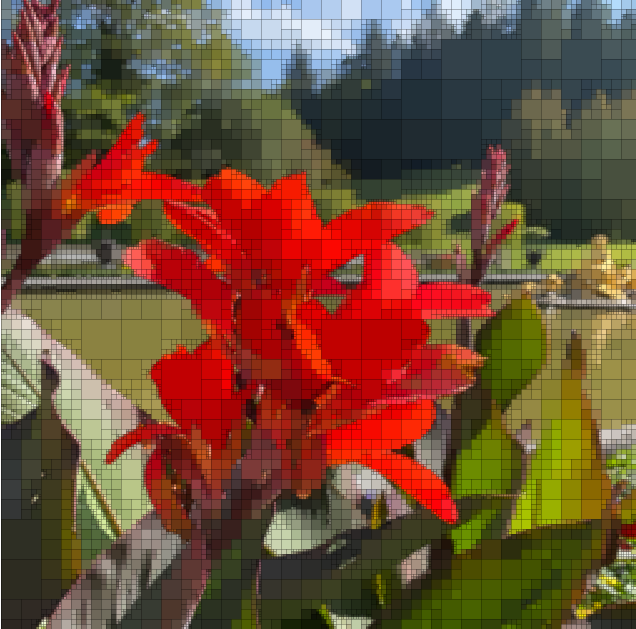
\includegraphics[width=6cm]{quadtreebildcompressionBlume.png}
    \caption{Quadtree Bild Kompression}
    \label{quadtreeImageProcessing}
    
    \end{center}
    \end{figure} \footnote[1]{Fogleman, Michael: Quads, https://www.michaelfogleman.com/static/quads/, aufgerufen am 5.06.2021}

\pagebreak

\subsubsection{Aufbau}

Der \qt hat einen ähnlichen Aufbau wie die binären Bäume. Was in unterscheidet ist die Anzahl der nachfolgenden Knoten, was bereits in \ref{Quadtree} erwähnt wurde.
Was ihn weiter abgrenzt ist der key value im Knoten, der im \qt gesplittet wird. Demzufolge besitzt der z.B. Point-\qt einen x-value und y-value. \newline
Für diese Arbeit wurde ein Point \qt implementiert. Die anderen Ansätze haben einen ähnlichen Aufbau, unterscheiden sich jedoch sowohl im Unterteilungskriterium als auch in dem aasgespeichert wird, weil neben dem Punkt z.B. ein Polygon weitergegeben wird.
\newline
Zuerst muss eine Fläche definiert werden, worin wir die Daten, in meinem Code Beispiel Punkte, einfügen und speichern. Dies erfolgt durch die struct class \lstin{struct rectangle}.
\begin{lstlisting}
 struct Rectangle{
    // point_t point; 
    randPoint_t point;                                                       
    double width;
    double height; 
};
typedef struct Rectangle rectangle_t;
\end{lstlisting}
Wir benötigen einen Punkt, welcher sich in der Mitte des Quadranten befindet, dieser wird für die Teilung genutzt. Außerdem wird die Weite und Höhe definiert. 
Was im späteren Verlauf nicht vegessen werden darf, ist die Halbierung der beiden Grenzen, da der Zentrumspunkt der Ursprung ist und wie im Koordinatensysten positive als auch negative Werte besitzt. 
Darauf werde ich noch etwas genauer in einem späteren Abschitt eingehen. 
\newline
Da ich mich für den Point \qt entschieden habe, darf die Punkte Klasse nicht fehlen. Diese besteht aus einem x-value und einem y-value. Ich habe mich für den Datentyp double entschieden, aus dem Grund das größere Zahlen errreicht werden können. Bei bei der Teilung der Quadranten können Kommazahlen entstehen, welche durch den Datentyp \lstin{int} einfach aufgerundet werden und somit Werte verfälscht werden. 
Um eine gewisse Anzahl an Punkte zu erreichen wurde die Random Function \lstin{rand()} genutzt.  
 
\begin{lstlisting}
    struct RandomPointGenerated{
    double xValue; 
    double yValue; 
};
typedef struct RandomPointGenerated randPoint_t;
\end{lstlisting}
In der Quadtree Struktur wird eine \fett{boundary} definiert, welche vom Datentyp \lstin{rectangle_t} ist. Somit besteht die Boundary aus einem Mittelpunkt, Breite und Höhe. Zusätzlich wird ein Array initialisiert des Datentyps \lstin{randPoint_t} mit einer vorbestimmten maximalen Kapazität. Bei erreichen der maximalen Kapazität wird wann der Quadtree geteilt. 
Die maximale Kapazität habe ich bereits am Anfang mit \lstin{#define capacity_of_Points 2} vordefineriert. Somit wird geteilt, wenn mehr als 2 Punkte im Quadranten sind. Um bestimmen zu können wie viele Punkte im Quadranten gerade vorhanden sind, wird eine variable \lstin{n_points} initialisiert vom Datentyp \lstin{int}.
Nun kommen wir zu einem der wichtigsten Punkte bei der Implementierung des \qts, sprich den children nodes oder auch inneren Knoten. \newline
Anstatt einen Speicherplatz komplett zu reservieren, greifen wir auf Pointer zurück. Dies ermöglicht es, leichter Referencen zu generieren und ist außerdem speicherfreundlich. Entsprechend des Aufbaues des \qts , haben wir vier Nodes. Um die Position genauer bestimmen zu können, werden diese nach den Himmelsrichtungen benannt. Es ist aber auch möglich sie durchzunummerieren, das kann aber schnell zu Verwirrung führen. 
Daher habe ich mich für die andere Variante entschieden.\newline
Bei meiner Implementierung wird der \qt in gleich große Quadranten geteilt, und es entstehen die neuen Quadranten \nw , \noea , \sw , \se. 

\begin{lstlisting}  
    struct QuadTree{
    //the boundary of the node
    rectangle_t boundary;                                     
    randPoint_t points[capacity_of_Points];                  
    int n_points;                                            
    //childrenNodes
    struct QuadTree *northWest;                             
    struct QuadTree *northEast; 
    struct QuadTree *southWest; 
    struct QuadTree *southEast; 
};
typedef struct QuadTree QTree_t; 
\end{lstlisting}

\subsubsection{CreatingQuadtree Funktion}
Um die Unterteilung in die jeweiligen Quadranten des \qt zu ermöglichen, müssen wir erst einmal Speicher für den parentQuadTree reservieren,was wir durch \lstin{malloc()} erreichen,welcher den Speicherplatz so anpasst, das nur der Speicher reserviert wird. 
Die Werte werden auf \lstin{NULL} initialisiert, damit es im späteren Verlauf zu keinem Fehler kommt. 
Wenn es zu einem Speicherfehler kommen sollte, wird ein Error geprinted und das Programm gestoppt. 
Wir haben am Anfang noch keine Punkte im \qt, deswegen wird auch das Array \lstin{n_points = 0;} gesetzt. 
Somit werden alle Werte mit dem Startwert Null versehen und sobald ein \qt initialisiert wird, werden die jeweiligen Werte übernommen. Normalerweise würde ein Konstruktor definiert werden, in der Programmiersprache \lstin{C} ist dies aber nicht realisierbar.

\begin{lstlisting}

    QTree_t *createQuadtree(double centerX, double centerY, double width, double height){
    QTree_t* result = malloc(sizeof(QTree_t));
    if(result == NULL){
        printf("Malloc returns NULL. \n EXIT! \n");
        exit (1); 
    }
    result->northWest = NULL;               
    result->northEast = NULL; 
    result->southWest = NULL; 
    result->southEast = NULL;
    result->n_points = 0; 
    result->boundary.height = height; 
    result->boundary.width = width; 
    result->boundary.point.xValue = centerX; 
    result->boundary.point.yValue = centerY; 

    return result; 
}
\end{lstlisting}

\subsubsection{insertPoint funktion}

Es folgt die \lstin{insertThePoint} Funktion für das Einfügen der Punkte im \qt. Dazu brauchen wir zum einem einen parent QuadTree \lstin{QTree_t *quadTree} sowie Punkte \lstin{randPoint_t randPoint}.\newline
Zunächst wird die Grenze oder boundary definiert und initialisiert mit den neuen x und y werten sowie der Höhe und Breite.

\begin{lstlisting}
    double cx = quadTree->boundary.point.xValue; 
    double cy = quadTree->boundary.point.yValue; 
    double w = quadTree->boundary.width; 
    double h = quadTree->boundary.height;
\end{lstlisting}
Da ich die Random Function \lstin{rand()} nutze und nur in einem bestimmten Bereich die x und y Werte liegen sollen, müssen noch die Grenzen bestimmt werden. Meine Überlegung war, dass der minimale Wert die negative Hälfte der Breite ist und der maximale Wert die positive Hälfte der Breite.
Durch dies werden die Punkte immer in der Boundary liegen. 
\begin{lstlisting}
    double min_range = -w/2; 
    double max_range = w/2; 
\end{lstlisting}
Falls es doch zu einer Überschreitung der Boundary kommt, wird diese mit einer \lstin{if} Abfrage abgefangen. Das Programm würde sich in diesem Fall beenden. 

\begin{lstlisting}
    if(!(randPoint.xValue >= cx - w/2 && randPoint.xValue <= cx + w/2 && randPoint.yValue >= cy - h/2 && randPoint.yValue <= cy + h/2)){
        printf("Error! The Point is not in the Boundary of the Quadtree!\n");
        exit(1); 
    }
\end{lstlisting}
Damit der \qt nicht mehr weiter unterteilt wird wenn die Breite oder die Höhe null sind und  Punkte mit null Werten entstehen, wird dieser Fall ebenfalls mit einer \lstin{if} schleife abgefangen. 
\begin{lstlisting}
    if(quadTree->boundary.width == 0.0 || quadTree->boundary.height == 0.0){
        printf("The quadtree cant be divided anymore! \n");
        exit(1); 
    }
\end{lstlisting}
Nun kommen wir zu der \lstin{for} schleife, in welcher sowohl die Unterteilung der Node erfolgt als auch der Generierung der Punkte.\newline
Da ich den \lstin{double} Datentyp verwende und keine \lstin{int} Werte als Ausgabe bekommen möchte wenn ich den modulo Operator verwende, habe ich die \lstin{fmod()} Funktion verwendet. Hiermit wird der Rest von den zwei \lstin{double} Werten zurückgegeben unter Berücksichtigung der Nachkommazahlen. 
\begin{lstlisting}
    randPoint.xValue = fmod(rand() , quadTree->boundary.width/2); 
    randPoint.yValue = fmod(rand() , quadTree->boundary.height/2); 
\end{lstlisting}
Da ich in der Grenze des \qts bleiben möchte, habe ich die Werte, welche x annehmen kann auf die Hälfte der Breite gesetzt. 
Mithilfe einer Weiteren \lstin{if} schleife werden die Punkte abgefangen, die gleich null sind: 
\begin{lstlisting}
    if(!(randPoint.xValue != 0 && randPoint.yValue != 0)){
        printf("Sorry cant be inserted!\n");
        exit(1);
\end{lstlisting}
Die Punkte werden anschließend in das Array gespeichert, wenn die maximale Kapazität nicht erreicht wurde. 
\begin{lstlisting}
    if(quadTree->n_points < capacity_of_Points){
        printf("direct adding to tree...\n");
        quadTree->points[quadTree->n_points++] = randPoint; 
\end{lstlisting}
Sobald die Kapazität erreicht ist, wird der Quadrant unterteilt. Wenn er noch nicht unterteilt wurde, erfolgt dies zuerst. Danach wird bestimmt wo der Punkt sich genau befindet. Wenn der x Wert und der y Wert positive sind, wird der punkt in northEast hinzugefügt.
Ist der x Wert positiv, der y Wert jedoch negativ wird der Punkt in southEast hinzugefügt. Sollte der x Wert negativ sein, der y Wert aber positiv, befinden wir uns in northWest. sind beide Werte negativ, wird der Punkt in southwest hinzugefügt.  
\begin{lstlisting}
    if(quadTree->northEast == NULL){
        printf(" \n node will be subdivided..\n");
        subdivideNode(quadTree);
        }
            int positiveX = randPoint.xValue - cx >= 0; 
            int positiveY = randPoint.yValue - cy >= 0; 
        if(positiveX){
            if(positiveY){
                    printf("Point: %.2f/%.2f \n", randPoint.xValue, randPoint.yValue);
                    printf(" Point in northEast\n");
                    insertThePoint(quadTree->northEast, randPoint);
            }else{
                    printf("Point: %.2f/%.2f \n", randPoint.xValue, randPoint.yValue);
                    printf("Point in southEast\n");
                    insertThePoint(quadTree->southEast, randPoint);
            }
        }else{
            if(positiveY){
                    printf("Point: %.2f/%.2f \n", randPoint.xValue, randPoint.yValue);
                    printf("Point in northWest\n");
                    insertThePoint(quadTree->northWest,randPoint);
            }else{
                    printf("Point: %.2f/%.2f \n", randPoint.xValue, randPoint.yValue);
                    printf("Point in southWest\n");
                    insertThePoint(quadTree->southWest, randPoint);
\end{lstlisting}


\subsubsection{subdivideNode Funktion}
Für die Unterteilung des parent \qts wurde eine eigene Funktion implementiert, welche die node in ihre children Nodes teilt. Wie der parent Node werden die Quadranten mit einem neuen Mittelpunkt und neuen Breiten und Höhen definiert.
\begin{lstlisting}
    // boundary: x - w/4 , y - h/4 , w/2 , h/2    northWest
    // boundary: x + w/4 , y - h/4 , w/2 , h/2    northEast
    // boundary: x - w/4 , y + h/4 , w/2 , h/2    southWest
    // boundary: x + w/4 , y + h/4 , w/2 , h/2    southEast
\end{lstlisting}
Für die Berechnung der neuen Boundary Werte der neuen Quadranten, müssen die Abstände zu dem Zentrumspunkt neu berechnet werden ebenso die neue Höhe und Breite. 


\subsubsection{rangeQuery Funktion} \label{QuerySuche}
Diese Funktion ist dafür da, dass in einem bestimmten Bereich alle Daten ausgegeben werden und nur in diesem Bereich gesucht wird. Damit wird Zeit gespart. Bei dieser Methode muss beachtet werden, dass die jeweilige Abfrageform in den jeweiligen boundarys ist. 
Wenn dies nicht der Fall ist, dann beginnt die Suche nicht. \newline
Außerdem wird ein Speicherort für die gefundenen Punkte benötigt, dies wird durch ein Array ermöglicht. 

\pagebreak
\subsection{\fett{\oc}}
Wie der \qt , ist diese Baumstruktur ähnlich aufgebaut wie der binäre Baum. Beim \oc gibt es jedoch nicht zwei oder vier children nodes, sondern acht oder gar keine. Dadurch findet diese Art von Struktur Anwendung im 3-dimensionalen Raum. 
Hier wird der Raum in jeweils 8 Octanten unterteilt und dies solange bis keine Teilung mehr möglich ist oder auch allgemein nicht mehr nötig ist. Dies erfolgt nach dem conquer and divide schema.  \ref{Octreeexample}
\begin{figure}[h]
    \begin{center}
    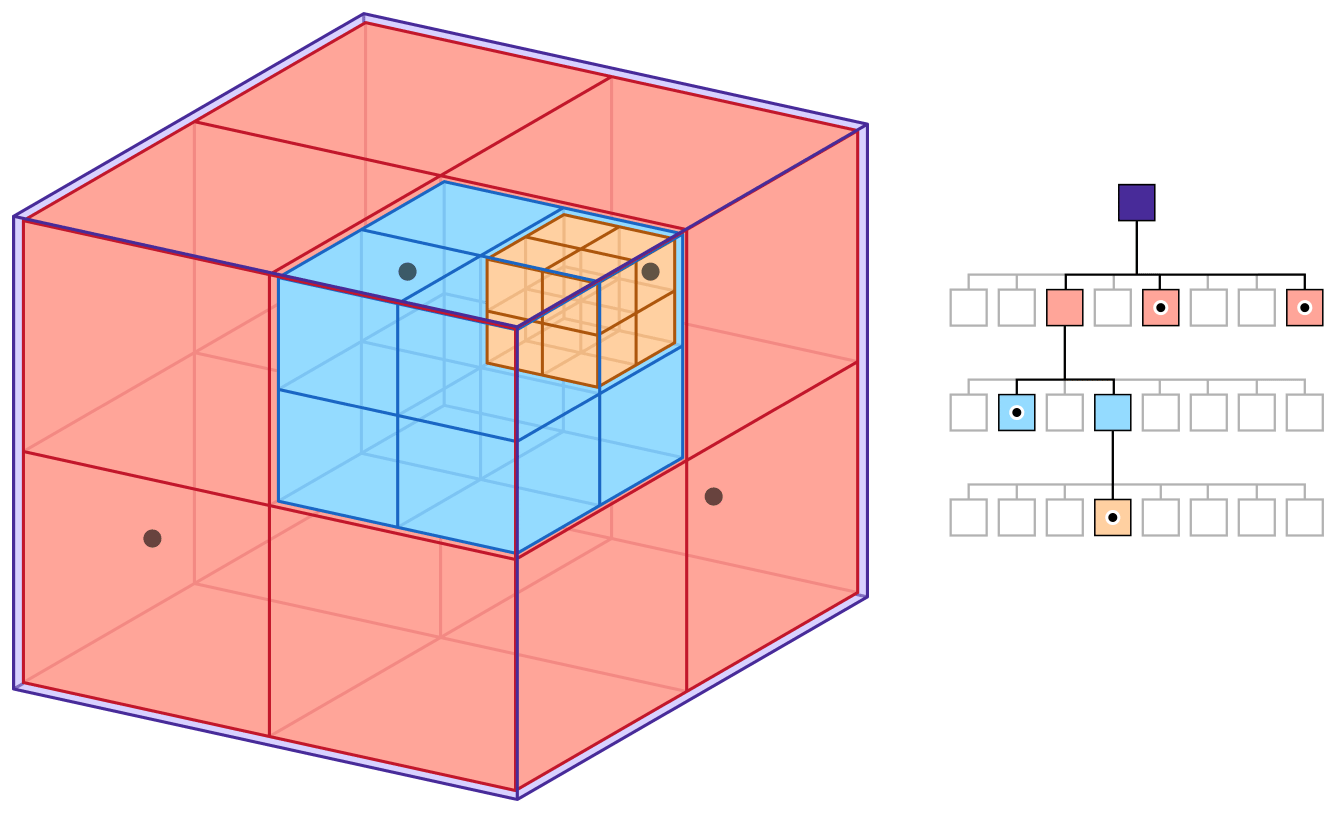
\includegraphics[width=6cm]{octree.png}
    \caption{Octree}
    \label{Octreeexample}
    
\end{center}
\end{figure}
Bei dem empty non empty \oc wird in den jeweiligen Knoten leer oder nicht leer gespeichert. 
Wenn der Knoten mit leer gekennzeichnet ist, wird verdeutlicht, das die Datenmenge, welche in diesem Octant ist, nicht weiter verabeitet werden muss. 
Sobald der Knoten nicht leer ist, wird die Datenmenge verarbeitet. 
Neben dem empty non empty \oc gibt es auch die variante Min max., in den jeweiligen Unterknoten werden dann jeweils die min und max werte hinterlegt, somit ist eine effizientere Suche gegeben. Durch die min max Werte können die Datenmengen schneller unterteilt werden und es muss nicht jeder Knoten untersucht werden. 
Der \oc findet Verwendung zum einen in 3D grafiken, zum anderen zur Bildrepräsentation, aber auch bei Raumindizierung wird der \qt verwedet. So können Partikel gruppiert werden und Zustandsschätzungen vorgenommen werden. Zusätzlich wird der \oc im marching cubes algorithm \footnote[1]{Lorensen, William E., and Harvey E. Cline. "Marching cubes: A high resolution 3D surface construction algorithm." ACM siggraph computer graphics 21.4 (1987): 163-169.} sowie im 3D game developement zur Kollisionserkennug genutzt. 
\newline
Vorteile des \ocs sind die effiziente Suche wie bei vielen anderen Strukturen, was einer der wichtigsten Punkte ist. Jedoch ist es schwer genaue Bestimmungen zu ermöglichen, da oftmals abgeschätzt wird wo genau sich z.b. die Partikel befinden. Wie bei vielen Baumstrukturen tendiert der \oc zur "nicht Ausbalancierung", womit viele unnötige Berechnungen erfolgen. 
Was sie von den \qt Strukturen unterscheidet ist die Möglichkeit, in einem 3D Raum Daten darzustellen wie Punkte aber auch Dreiecke. Mit dem \oc kann ähnlich wie beim marching cubes algorithm eine Isooberfläche generiert werden, jedoch ist diese Implementierung schwieriger mit der Struktur zu verwirklichen als hingegen der Algorithmus. 
Der marching cubes Algorithmus teilt den raum in gleich große Dreiecke, wohin gegen der \oc ungleichmäßig unterteilt. Dies hat den Nachteil, dass mehr Speicher benötigt wird und die Rechenzeit sich erhöht. Allerdings lassen sich damit Formen detalierter darstellen. \footnote[2]{https://stackoverflow.com/questions/15827385/what-is-the-difference-between-marching-cube-and-octree , aufgerufen: 10.10.2021}
\newline
Ray tracing ist ein weiteres Gebiet, in dem der \oc angewendet wird. Ray tracing wird verwendet um die Sichtbarkeit von Objekten zu berechnen. Durch dies können 3D-Szenen dargestellt werden, wie in Videospielen.  Es ist möglich mit dem \oc dieses zu Implementieren, jedoch gibt es eine Adaption der Datenstruktur, den \oc -R für effizientes ray tracing. Der Raum wird nicht mehr mit einem spatialen Mittelwert in voxeln geteilt, sondern durch einen Punkt. 
Anhand des \oc können die benötigten Tests für den ray tracing Algorithmus minimiert werden, indem berechnet wird, wo die Tests verlaufen und durch teilen des Raumes wird der Rechenbedarf minimiert.  \footnote[3]{Kyu-Young Whang et al., "Octree-R: an adaptive octree for efficient ray tracing," in IEEE Transactions on Visualization and Computer Graphics, vol. 1, no. 4, pp. 343-349, Dec. 1995, doi: 10.1109/2945.485621.}
Ich werde in meiner Arbeit nicht genauer auf diesen Algorithmus eingehen, allerdings kann ich diesen Artikel empfehlen welcher sich damit genauer beschäftigt. \cite{RaytracingOctree}

\subsection{\fett{\kd}}
Bei dieser Datenstruktur handelt es sich um einen ausbalancierten Suchbaum. In diesem werden Punkte aus dem $\mathbb{R} ^k$ Raum gespeichert. Jeder Knoten stellt hier den k-dimensionalen Punkt dar. 
Der \kd tree wird für ray tracing und nearest neighbour search benutzt. Zudem können sogenannte Point Clouds generiert werden. 
Die Teilung in Subsektionen erfolgt nach Bestimmung eines Kriteriums. Bei Punkten könnte einer gewählt werden, welche sich in der Mitte des Quadranten oder Rechtecks befindet. Auf der linken Seite würden dann alle Werte dargestellt werden, welche kleiner als der Kriteriumspunkt sind, auf der rechten alle die größer sind. Außerdem wird abwechselnd das Kriterium geändert. Somit wenn als erstes nach dem Mittelwert der x Achse gesucht wurde, wird als nächstes nach dem Mittelwert der y Achse gesucht. Damit können Daten effizienter unterteilt werden.  
\newline
Es gibt verschiedene Arten dieser Struktur, zum einenen Homogene als auch inhomogene Trees. Nebenen Punkten ist auch die Speicherung von Rechtecken möglich. Die Speicherung der Punkte in nur den leafs/ blättern ist auch ausführbar. Wie beim \oc  können auch nur min und max Werte in den nodes gespeichert werden.
Durch die bessere Apassung und das abwechseln der jeweiligen divide Kriterien wird die Struktur besser unterteilt und es folgt, das die Knoten dieser Baumstruktur besser ausbalancierbar sind als die des \qts. Im \qt wird nur nach einem Kriterium unterteilt. 
Es gibt verschiedene Möglichkeiten, den \kd aufzubauen. Da wir entlang der Achse gehen, haben wir dadurch viele Möglichkeiten zu starten. 
Bei einem 2-d tree würde die parent node erst die x Achse als Teilebene nutzen, anschließend die y Achse und in diesem Ablauf bis zur Endbedingung durchlaufen. 
Die Punkte werden unter Brücksichtigung des berechneten Medians eingefügt.  Durch diesen Ansatz kann der \kd gut ausbalanciert werden, da durch die Berechnung des Medians der entsprechenden Punkte es zu keinem großen unterschied in den Bereichen kommt. 
Die Unterteilung der leaves unterläuft meist,das nach links alle kleineren werte als der Median Wert links eingefügt werden, recht alle Daten die größer sind.  
\newline    
\fett{pointlist:} { (10,3) (6,3) (11,4) (3,2) (4,8) (2,1), (4/2) } 
\newline

\begin{tikzpicture}[sibling distance=14em,   
    every node/.style = {shape=rectangle, rounded corners,
      draw, align=center,
      top color=white, bottom color=blue!10}]]
    \node {Start Value: X: 10, Y: 3}
      child { node {less than X value: (6 / 3)}
            child {node {less than Y value : (3/2)}
                child{node {less than X value : (2/1)}} 
                child{node {greater than X value : (4/2)}}}
            child {node {greater than Y value: (4/8)}}}
      child{node {greater than X value: (11,4)}};
\end{tikzpicture}
In der Grafik wird einer beispielhafter Aufbau eines \kd dargestellt. Der erste Punkt der eingefügt wird ist (10/3). Sobald der zweite Punkt hinzugefügt wird, werden die X-werte verglichen. (6,3) ist kleiner und wird auf der linken Seite eingeordnet.
(11,4) hat einen größeren X wert und wird somit auf der rechten Seite angeordnet. Die nächsten hinzugefügten Punkte (3,2) und (4,8) haben jeweils einen kleineren X-Wert. Somit werden sie auf der linken seite eingeordnet. Dort ist aber schon der Punkt (6/3).
Diesmal wird der Y-Wert der beiden Punkte mit dem (6/3) Punkt verglichen. Damit ergibt sich, dass (3,2) wiederrum links eingeordnet wird da der Y-Wert kleiner ist und (4,8) rechts zugeordnet wird. 
(2,1) und (4/2) haben sowohl einen kleineren X-Wert gegenüber (10/3), als auch Y-Wert zu (6/3). Nun wird wieder der X-Wert der beiden mit (3/2) betrachtet und richtig eingeordnet. Nun haben wir schematisch einen beispielehaften Aufbau eines \kd. 
\newline
Ein Anwengungsgebiet für den \kd ist die nearest neighbour search.  Dies ist ein Algorithmus in welchem in der Nähe eines bestimmten Startwertes der nächstgelegene Punkt gsucht wird. Vorteil an diesem ist ,dass die Suche effizienter und schneller ist, indem nicht jede node durchlaufen werden muss. 
Durch die Abwechslung der Rahmenbedingungen ist der \kd besser für die suche von Daten geeignet als der \qt. Außerdem ist er besser ausbalanciert, was eins der Probleme bei dem \qt ist. 

\pagebreak

\section{Variationsmöglichkeiten} \label{Varianten}

\subsection{Zusammenfassung}
Wie bereits in den Kapiteln davor behandelt, ist es möglich die Strukturen unterschiedlich zu implementieren. 
Der \qt kann in gleich große Formen geteilt werden, was bei dem Image processing von Vorteil ist. Zumal wir das Bild fragmentieren wollen und dieses gleichmäßig sodass die jeweiligen children nodes immer die gleiche Breite und Höhe haben. Anderseits können die jeweiligen Grenzen angepasst werden, wenn in einem Raum Punkte an einem Ort sehr angereichert sind, würde es wenig Sinn machen gleichmäßig zu unterteilen. 
Dies würde nur zu große leere Quadtranten führen, wodurch sowohl der Speicher für die leeren Blättern verschwendet wird, als auch es zu einem unausbalancierten Baum. 
\newline
Wenn wir den Ansatz verwenden, wo wir die Quadraten immer mit einer bestimmten Bedingung unterteilen, kann der Speicher effizienter verwenden werden.  Somit sollte immer darauf geachtet werden, ob es sich in dem Fall anbieten würde, diese Unterteilung zu benutzen.
Das gleiche gilt bei dem Octree. Wenn dort im 3D raum Punktmengen angehäuft sind, wird sich das Voxel öfters teilen, allerdings führt das schnell zu ausbalancierten Bäumen. 

\subsection{Programmbibliotheken}
 
Für den \qt gibt es die Libary \lstin{quadtree-lib}, mit den Funktionen: hinzufügen von Elementen, entfernen von Elementen und weiteren Funktionen wie den Baum filtern. Hier wurde die Programmiersprache \fett{CoffeeScript} verwendet. \footnote[1]{https://www.npmjs.com/package/quadtree-lib ,aufgerufen am 01.10.2021}
Eine weitere Implementierung in der Programmiersprache \fett{Python} ist der \lstin{Pyqtree}. Genutzt wird diese Art von \qt zur Raum Indezierung bei GIS Systemen oder Rendering. \footnote[2]{https://pypi.org/project/Pyqtree/, aufgerufen am 10.06.2021}
Für das Umwandeln von Point Cloud Daten in die Baumstruktur \oc ist die Point Cloud Libary \lstin{pcl_octree} in \fett{C++} nützlich. Mit dieser können auch effiziente nearest neighbor Suchen genutzt werden. Für ray tracing und shadow casting kann die Bibliothek \lstin{pyoctree 0.2.10} genutzt werden. \footnote[3]{https://pypi.org/project/pyoctree/ , aufgerufen am 12.06.2021}
Auch für den \kd ist eine PCL libary vorhanden. \lstin{pcl_kdtree} kann für die schnelle nearest neighbor suche verwendet werden. Diese Libary ist in der Programmiersprache \fett{C++}. \cite{PointCloudLibary}
Dies sind nur ein paar Beispiellibaries von Vielen.



\pagebreak

\section{Komplexität der jeweiligen Baum-Daten Strukturen}
In diesem Kapitel geht es um die Komplexität der jeweiligen Strukturen. Somit um den Ressourcenverbrauch bei der Verwendung der jeweiligen Algorithmen. Diese ist abhängig davon, wie die die Datenstrukturen aufgebaut sind und wie viele Daten sie verarbeiten und speichern müssen. 
Zudem kommt hinzu, wie gut die Implentierung umgesetzt wurde. Zwar wird immer vom besten Ergebnis ausgegangen, hingegen wird dieses Ergebnis nie komplett ereicht werden, da viele Faktoren dies verhindern. Zum einen ist es abhängig von der Hardware, ob ich Hochleistungsrechner benutzt wird oder nur ein Laptop.
Zum anderen kommt hinzu, dass die Implementierung vielleicht fehlerhaft ist. Diese Faktoren dürfen nicht unterschätzt werden. 


\subsection{\qt}

Betrachten wir einmal die hierarchische Struktur des \qt. Bei einer anzahl von n= 100 und n= 10000 beträgt die allgemeine Rechenzeit $log$ n. In einem worst case Szenario würde die Rechenzeit gleich der Node anzahl stehen. Dies wäre der fall wenn der Baum nicht ausbalanciert ist und bedeutet wir hätten nur eine node mit einer großen tiefe, was zu eienr linked List führen würde.
Allgemein gubt es eine Formel die den Aufwand berechnet: 
\begin{equation*}
    \fbox{C  $_n^d$ $=$ $\frac{a}{b}$ $log$ n} 
\end{equation*} 
Nun werfen wir einen Blick auf die Suchfunktion mit s Punkten aus D Koordinaten. \newline
\begin{equation*}
    \fbox{Q$_n^{(s,d)}$ $=$ $\theta^{(1- \frac{s}{d})}$n  }
\end{equation*}
Dies wäre die Berechnung der Komplexität für den perfekten Baum. Jedoch wird die Baumstruktur nie perfekt sein. 
Deswegen die neue Formel, in der die Abweichung mit einbezogen wird. 
\begin{equation*}
    \fbox{ Q$_n^{(s,d)}$ $=$ $\Theta^{(1- \frac{s}{d} + \theta\frac{s}{d})}$n }
\end{equation*}
Die Korrektur Funktion $\theta(x)$ im Exponenten ist die Lösung der Gleichung mit 
\begin{equation*}
    \fbox{$\theta \in [0,1]$ :  $(\theta + 3 -x)^x(\theta + 2 - x)^{1-x} -2 = 0$ }
\end{equation*}
Allgemein kann gesagt werden, dass die Kosten, unabhängig ob der \qt erfolgreich war oder nicht eine Komplexität von $\log n + O(n)$ hat siehe \cite[S.475ff]{quadtree} .
Das worst case dieses Alogrithmuses wäre der Fall, dass die Anzahl aller Nodes gleich der Ausführungszeit ist somit also $O(n)$. \footnote[1]{Flajolet, Philippe, et al. "Analytic variations on quadtrees." Algorithmica 10.6 (1993): 473-500.}

\subsection{\oc}

Der Rechenaufwand funktioniert bei dem \oc genauso wie bei dem \qt . 
Betrachten wir die find function haben wir einen Rechenaufwand von $O(\log2 $ N). 
Ähnlich sieht es bei der insert und der search Funktion aus. Diese besitzen den gleichen Aufwand $O(\log2 $ N).
Das worst case szenario wäre hier auch $O(n)$. 
Wenn wir die Raumkomplexität betrachten, und k definiert ist als die Anzahl der Punkte im Raum, kommen wir auf die Formel:
\begin{equation*}
    \fbox{$O(k \log2 N) $}  
\end{equation*}

\subsection{\kd}

Der Aufwand allgemein ist $O(n \log n)$, wie auch bei den beiden anderen Datenstrukturen ist der worst case hier $O(n)$. 
einen Punkt in einem balancierten \kd hinzuzufügen braucht um die Zeit $O(\log n)$ . einen Punkt zu entfernen $O(\log n)$. 
Dem Baum zu durchsuchen pro range point dauert um die $O(\log n)$, somit ungefähr $O(n \log n)$ im Ganzen betrachtet. \footnote[1]{vgl. Flajolet, Philippe, et al. "Analytic variations on quadtrees." Algorithmica 10.6 (1993): 473-500.}

\pagebreak

\section{Zusammenfassung}
In den vorherigen Kapitel habe ich bereits die Datenbaum Strukturen vorgestellt und erklärt. Ich werde diese Informationen nochmals kurz zusammenfassen und den \qt mit den \oc und \kd Strukturen vergleichen. 
\newline    
Was alle drei Strukturen miteinander vereint, ist die Reihenfolge der Datenmengen. Sie alle besitzen eine Root und anschließend folgen die Knoten mit den Daten. Die Root wird immer an erster Stelle stehen, da die Knoten von dieser Daten "erben". Nun gibt es natürlich Fälle wo dies nicht zutrifft, doch wir werfen hier nur einem Blick auf die vorgestellen Bäume. 
\newline
Betrachten wir nun die Art der Unterteilung der Bäume. Diese ist abhängig von der Datenmenge, welche gespeichert wird. Nehmen wir das Beispiel mit Punkten in einem Raum. Hierfür würde die Unterteilung des Raumes bei dem \qt und \oc ähnlichen erfolgen. 
Der Unterschied ist die Dimension des Raumes. Im \qt wird ein 2D-Raum unterteilt sobald die maximale Kapazität der Punkte erreicht ist. Der \oc ist eine Weiterentwicklung des \qt und unterteilt sich, sobald auch die maximale Kapazität erreicht sein sollte, nur befinden wir uns im 3D Raum. 
Bei dem \kd erfolgt die Unterteilung des Raumes durch das Suchen des Medianpunktes und anschließend der Unterteilung der Punkte mit Berücksichtigung, dass die Achse abgewechselt wird.  \newline
%freie bereichen
Bei der Unterteilung der Bäume kommt es oftmals zu dem Problem, dass bei einer dichten Anzahl von Punkten viel unterteilt wird, jedoch Räume entstehen die leer sind. Es kann zu eienr mangelnden Ausbalanciertheit kommen.
Dieses Problem haben vor allem der \qt und der \oc. Bei dem \kd wird durch den Algorithmus den dieser benutzt, dies weitestgehst verhindert. \newline 
%ausbalanciertheit 
Durch das Abwechseln der Achsen und der Berücksichtigung des Medianpunktes, hat der \kd wenig Probleme mit der ungleichmäßigen Verteilung der Unterbäume jedes Knotens. Dieses Problem tritt eher bei dem \qt und \oc auf. Durch Anpassung an diese Problem mit einer Gewichtung oder Balance der Knoten können aber auch diese relativ gleichmäßige Unterbäume generieren.\newline
%speicherorte 
Was sie alle verbindet ist die Art der Speicherung. Anhand von Pointern und \lstin{malloc()} werden Speicherorte reserviert und diese angepasst. 
Damit kann gesagt werden, dass der \oc viel Ähnlichkeit mit dem \qt hat und sich nur im Räumlichen unterscheidt. Der \kd hingegen hat viele Unterschiede zum \qt, und ist in manchen Situationen besser geeignet. Die Suche erfolgt schneller als im \qt , doch hängt der Nutzen von dem Anwendungsbereich ab, in welchem die Struktur verwendet werden soll. 

\pagebreak

\section{Eidesstattliche Versicherung}


Hiermit versichere ich, dass ich die vorliegende Arbeit selbstständig und ohne unerlaubte Hilfe angefertigt und andere als die in der Arbeit angegebenen Hilfsmittel nicht benutzt habe. 
Alle Stellen, die wörtlich oder sinngemäß aus anderen Schriften entnommen sind, habe ich als solche kenntlich gemacht sowie Abbildungen.

\includegraphics[scale=0.25,right]{unterschriftFürCseminar.png}
Freiberg, 17.10.2021 \hfill Siobhan Hönig

\pagebreak

\bibliographystyle{alpha}
\bibliography{references} % see references.bib for bibliography management

\end{document}